\subsection{Masa para croissants}
\label{sec:masa-para-croissants}

Basada en How to make bread por Emmanuel Hadjiandreou y \href{https://www.youtube.com/watch?v=hJxaVD6eAtc}{How To Make Proper Croissants Completely By Hand por Joshua Weissman}

\underline{Ingredientes}

\begin{itemize}
\item 250 gr de harina
\item 20 gr de azucar
\item 1 cucharadita de sal
\item 1$\sfrac{1}{2}$ cucharaditas de levadura
\item 125ml de agua tibia
\item 150 gr de mantequilla
\end{itemize}

\underline{Instrucciones}

\begin{enumerate}
\item Disolver la levadura en el agua tibia.
\item Mezclar la harina, la sal y el azúcar. Sólo hasta que este homogénea, no amasar en este paso.
\item Dejar reposar tapada en el refrigerador por 10 min y amasar jalando una parte de masa y empujándola en medio, 8 veces por todo el perimetro (ver Fig. \ref{fig:amasado-croissant}
\item Repetir el paso anterior, reposo y amasado, 3 veces más (un total de 4 veces).
\item Con la ayuda de papel encerado hacer un cuadrado con la masa de \Sim 15x15cm, y dejar por \Sim 8hrs en el refrigerador.
\item Con la ayuda de papel encerado formar un rectángulo de mantequilla homogéneo de \Sim 10x10cm.
\item Envolver la mantequilla con la masa como se muestra en la Fig. \ref{fig:envoltura-croissant} y dejarla reposar envuelta 1hr en el refrigerador.
\item Estirar un un rodillo como se muestra en la Fig. \ref{fig:doblado-croissant}, y doblar en tres. Trabajar sobre una superficie enharinada. Dejar reposar envuelta en el refrigerador por lo menos 30 min (más si se vuelve difícil de estirar).
\item Repetir el paso anterior 2 veces más (3 en total), girando la masa 90deg cada vez.
\item Dejar reposar envuelta en el refri por lo menos una hora antes de usar. 
\end{enumerate}

\begin{figure}
\centering
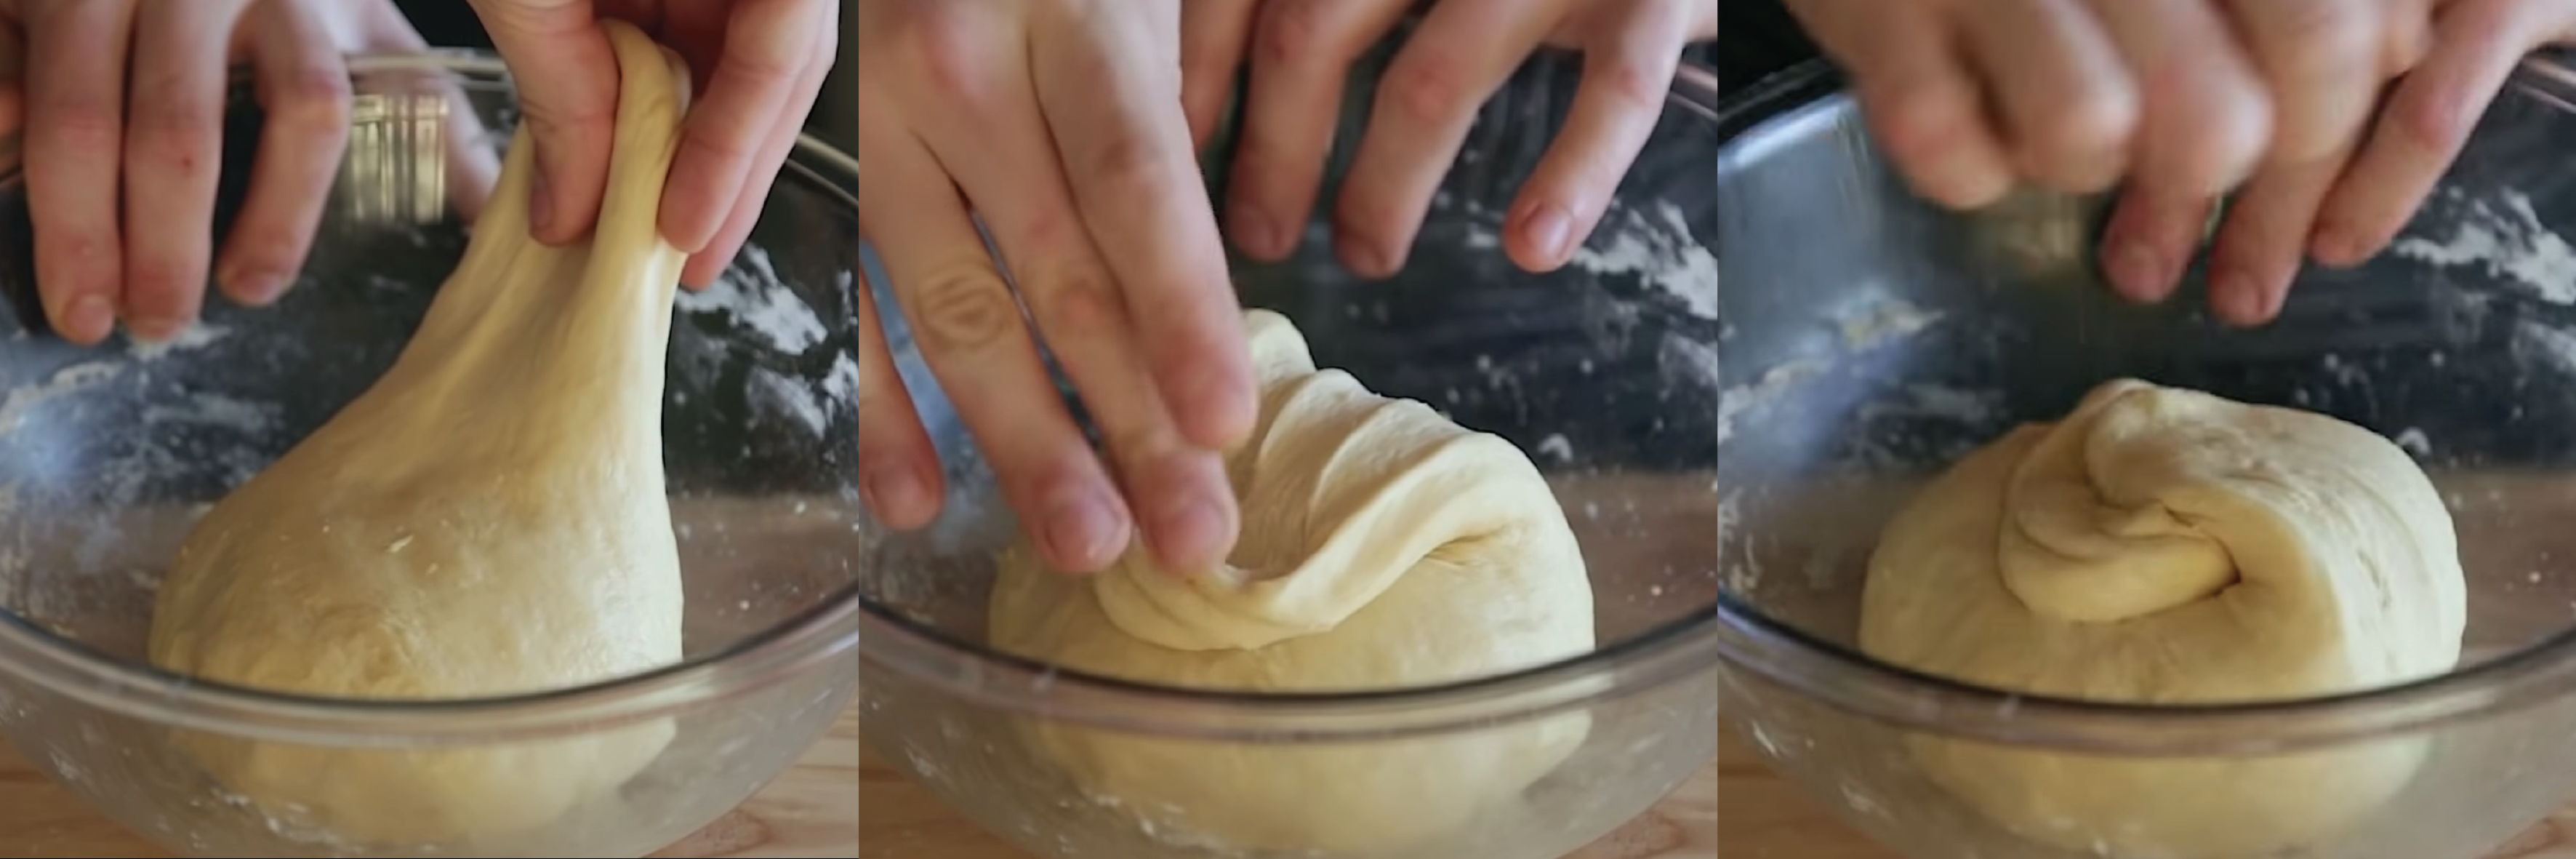
\includegraphics[width=1\textwidth]{recetas/croissants/figures/amasado-croissant.png}
\caption{Así se amasa la masa, 4 de estas! La de la imagen esta amarilla porque le añadieron huevo.}
\label{fig:amasado-croissant}
\end{figure}


\begin{figure}
\centering
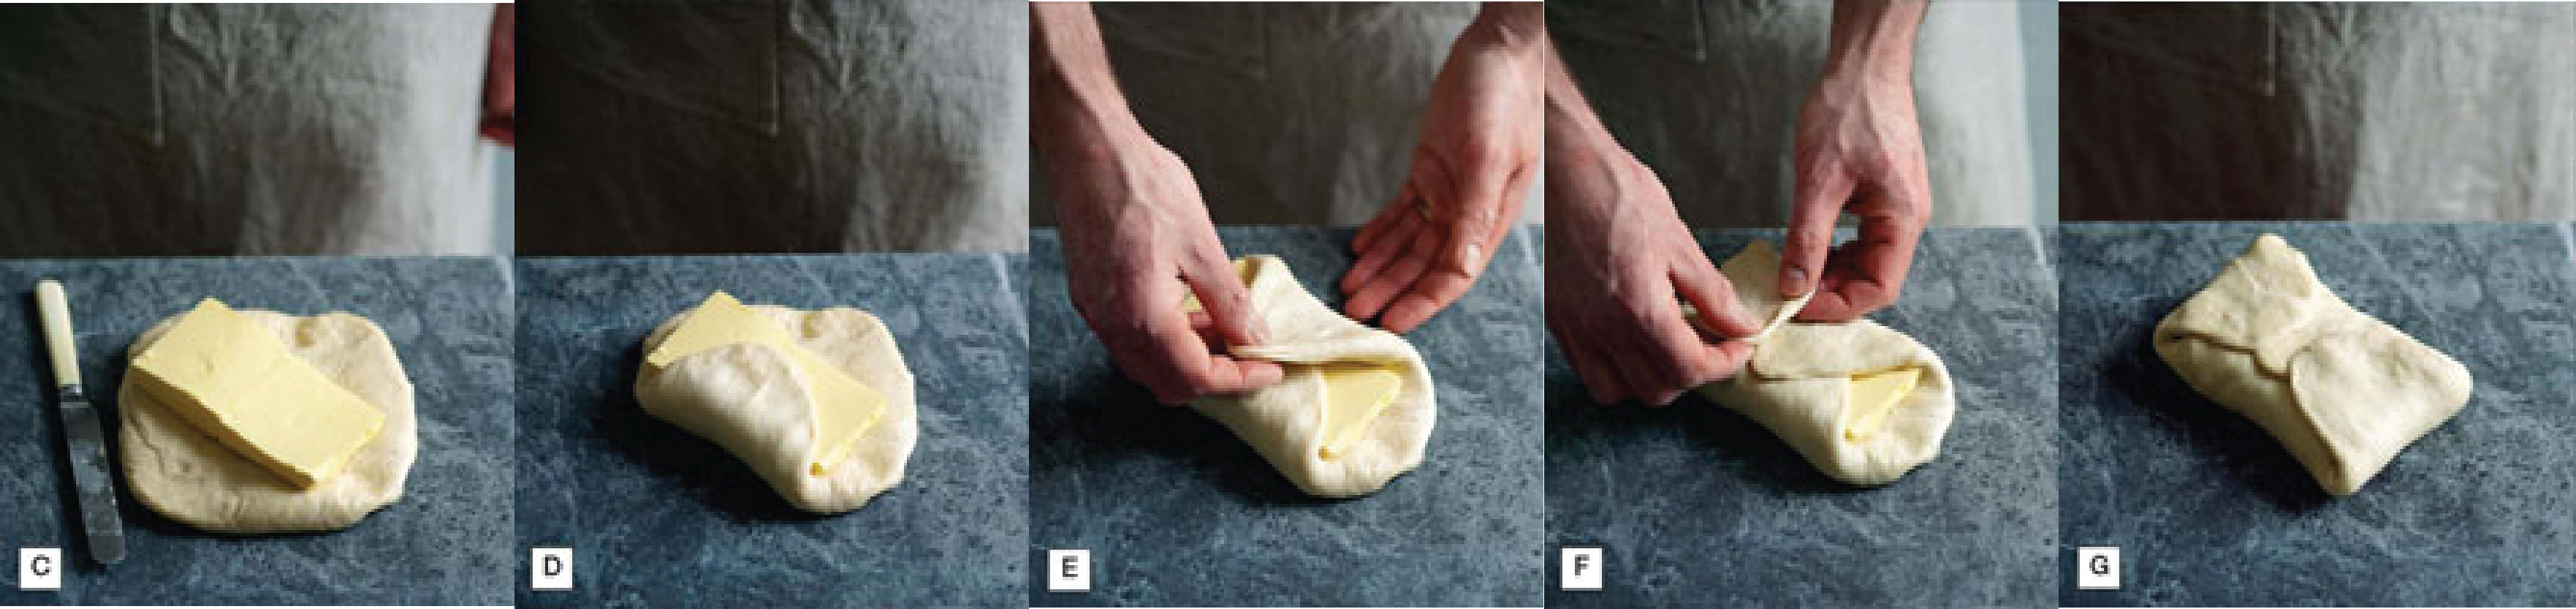
\includegraphics[width=1\textwidth]{recetas/croissants/figures/envoltura-croissant.png}
\caption{Así se envuelve la mantequilla! A mí me gustan más los cuadrados...}
\label{fig:envoltura-croissant}
\end{figure}

\begin{figure}
\centering
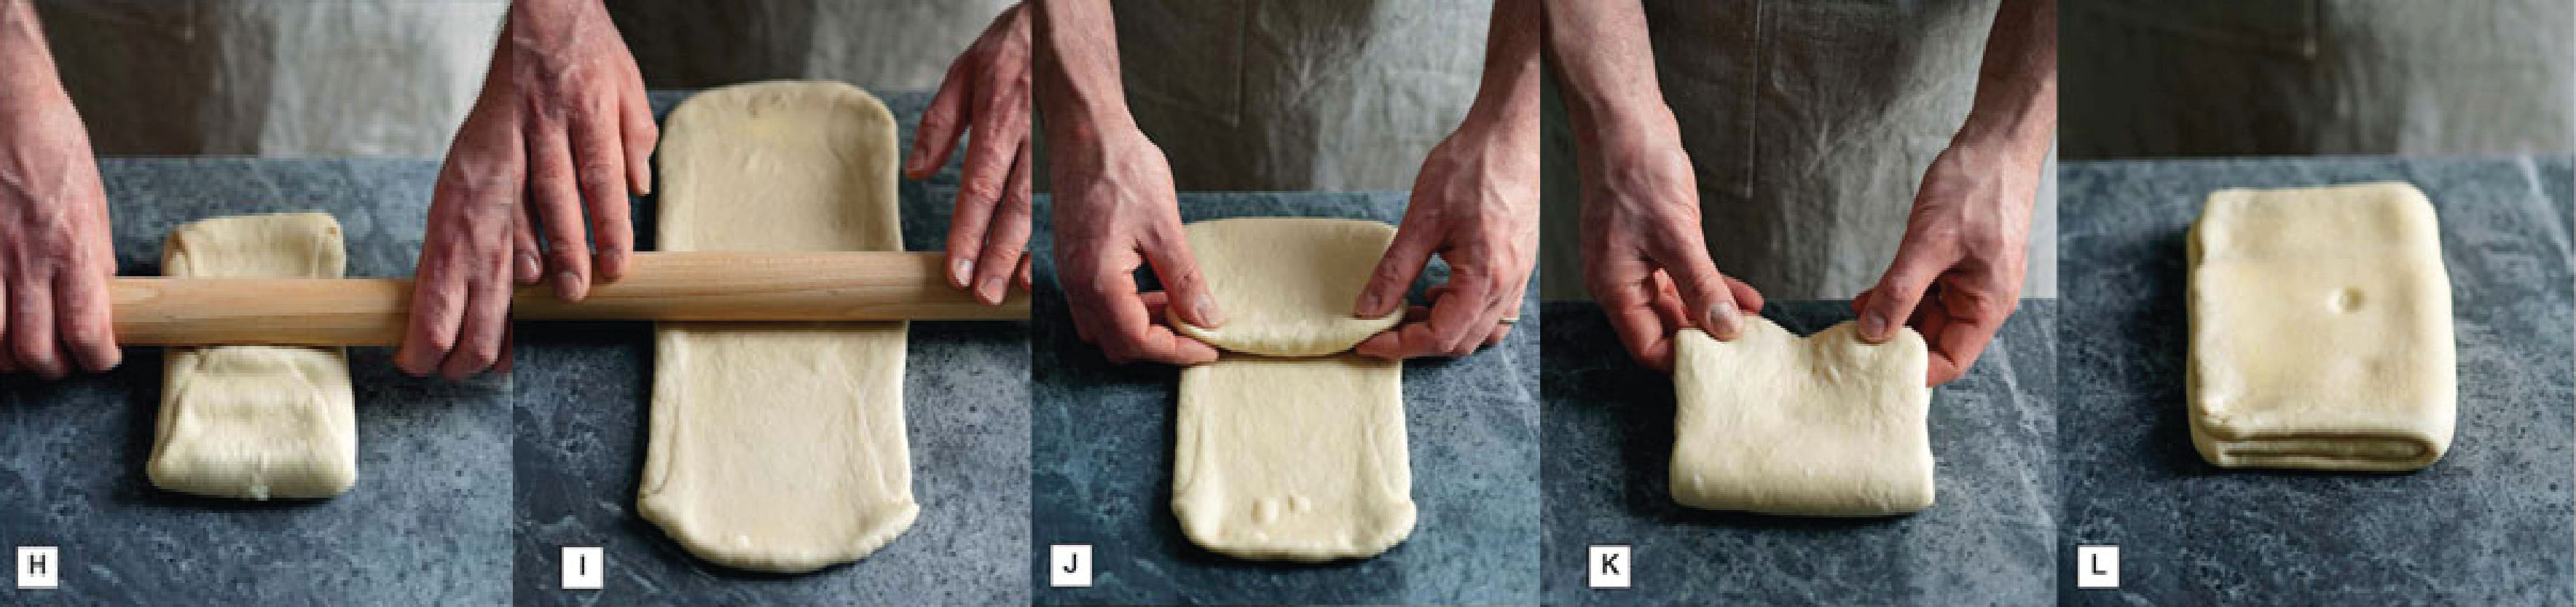
\includegraphics[width=1\textwidth]{recetas/croissants/figures/doblado-croissant.png}
\caption{3 de estas!}
\label{fig:doblado-croissant}
\end{figure}